\documentclass[./bab_4.tex]{subfiles}
\begin{document}
\section{Implementasi dan Uji Coba Sistem}

\subsection{Implementasi}
  \begin{enumerate}[label=\textbf{\arabic*.}]
    \item \textbf{Konfigurasi domain}
      \paragraph*{} Hal pertama yang perlu dilakukan adalah
      membuat konfigurasi domain, pada penelitian ini
      digunakan menggunakan cloudflare. 
      \begin{figure}[!ht]
        \begin{center}
          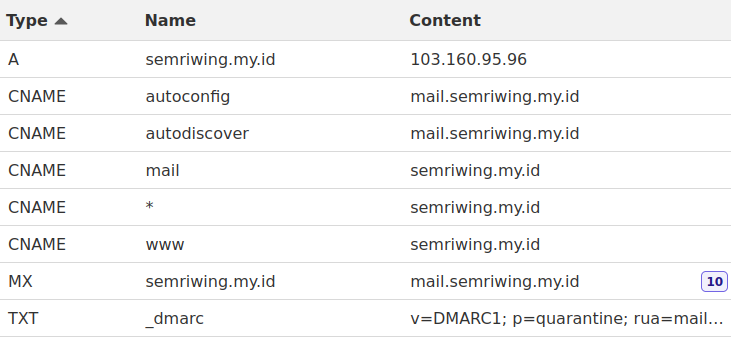
\includegraphics[width=0.95\textwidth]{dns1}
          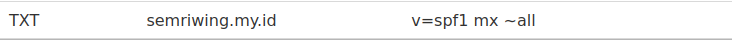
\includegraphics[width=0.95\textwidth]{dns2}
        \end{center}
        \caption{Konfigurasi domain}
        \label{konfdomain}
      \end{figure}
      
    \item \textbf{Instalasi Docker}
      \paragraph*{} Pada penelitian ini dilakukan
      instalasi Docker melalui repository dari Docker.
      Docker sebenarnya sudah tersedia di repository
      resmi dari Ubuntu server, tetapi Docker tersebut bukan
      versi yang terbaru.
      \DefTblrTemplate{caption-tag}{default}{\textbf{Tabel\hspace{0.25em}\thetable}}
      \DefTblrTemplate{contfoot-text}{default}{}
      \DefTblrTemplate{conthead-text}{default}{}
      \DefTblrTemplate{middlehead,lasthead}{default}{}
      \begin{longtblr}[caption= {Langkah instalasi Docker}]{hlines, vlines,
        column{1}={0.50\linewidth}, column{2}={0.50\linewidth}, rowhead=1} 
      \textbf{Perintah}   & \textbf{Keterangan}\\

        \texttt{sudo apt-get remove docker docker-engine docker.io
        containerd runc} & {Uninstall docker bawaan dari
        repository ubuntu}\\

        \texttt{sudo apt-get update} & {Memperbarui data
        repository}\\

        \texttt{sudo apt-get install ca-certificates curl gnupg
        lsb-release} & {Menginstall tools yang dibutuhkan
        untuk menambahkan repository}\\

        \texttt{sudo mkdir -p /etc/apt/keyrings} & {Membuat
        direktori tempat menyimpan keyring}\\

        \texttt{curl -fsSL
        \path{https://download.docker.com/linux/ubuntu/gpg} | sudo
        gpg --dearmor -o \path{/etc/apt/keyrings/docker.gpg}} &
        {Mengunduh keyring dan menambahkannya ke sistem}\\

        \texttt {echo  "deb [arch=\$(dpkg --print-architecture)
        signed-by=\path{/etc/apt/keyrings/docker.gpg}]
        \path{https://download.docker.com/linux/ubuntu}
        \$(lsb\_release -cs) stable" | sudo tee
        \path{/etc/apt/sources.list.d/docker.list} > /dev/null} &
        {Menambahkan url dari repository ke sistem}\\

        \texttt{sudo apt-get update} & {Memperbarui data
        repository}\\

        \texttt{sudo apt-get install docker-ce docker-ce-cli
        containerd.io docker-compose-plugin} & {Mengunduh
        dan menginstall docker}
      \end{longtblr}

      Setelah proses instalasi docker selesai, docker bisa
      dicoba dengan menjalankan perintah \texttt{docker}.

      \newpage

    \item \textbf{Menyusun Docker Compose}
      \paragraph*{}Langkah selanjutnya adalah membuat
      direktori baru, kemudian buat file docker-compose.yml.
      \begin{figure}[!ht]
        \begin{minted}[
            gobble=4,
            frame=single,
            linenos,
            breaklines
          ]{yaml}
    version: '3'
    services:
      php-apache:
        build:
          context: ./php-apache
        restart: "always"
        ports:
          - 80:80
          - 443:443
        volumes:
          - ./cert/semriwing.my.id:/var/imported/ssl/
          - ./www:/var/www/html:z
        depends_on:
          - 'database'
 
      database:
        image: mysql:8.0
        restart: "always"
        volumes:
          - ./mysql:/var/lib/mysql
        environment:
          TZ: ${TZ}
          MYSQL_ALLOW_EMPTY_PASSWORD: 'no'
          MYSQL_ROOT_PASSWORD: ${MYSQL_ROOT_PASSWORD}
          MYSQL_USER: ${MYSQL_USER}
          MYSQL_PASSWORD: ${MYSQL_PASSWORD}
          MYSQL_DATABASE: 'testdb'

        \end{minted}

        \caption{Isi dari file docker-compose.yml}
        \label{isicompose}
      \end{figure}

      \begin{figure}[!ht]
        \begin{minted}[
            gobble=4,
            frame=single,
            linenos,
            breaklines,
            firstnumber=last
          ]{yaml}
      mailserver:
        image: docker.io/mailserver/docker-mailserver:latest
        container_name: mailserver
        restart: "always"
        hostname: mail
        domainname: semriwing.my.id
        ports:
          - "25:25"
          - "587:587"
          - "143:143"
          - "465:465"
          - "993:993"
        volumes:
          - ./dms/mail-data/:/var/mail/
          - ./dms/mail-state/:/var/mail-state/
          - ./dms/mail-logs/:/var/log/mail/
          - ./dms/config/:/tmp/docker-mailserver/
          - ./cert/semriwing.my.id/:/tmp/dms/custom-certs/:ro
          - /etc/localtime:/etc/localtime:ro
        environment:
          - ENABLE_FAIL2BAN=1
          - SSL_TYPE=manual
          - SSL_CERT_PATH=/tmp/dms/custom-certs/fullchain.pem
          - SSL_KEY_PATH=/tmp/dms/custom-certs/privkey.pem
          - ONE_DIR=1
          - ENABLE_POSTGREY=0
          - ENABLE_CLAMAV=0
          - ENABLE_SPAMASSASSIN=1
        cap_add:
          - NET_ADMIN # For Fail2Ban to work

      webmail:
        image: docker.io/kouinkouin/snappymail:latest
        restart: "always"
        depends_on:
          - 'mailserver'

        \end{minted}
        \caption{Isi dari file docker-compose.yml (lanjutan)}
        \label{isicompose-lanjutan}
      \end{figure}

      \newpage 
    \item \textbf{Menjalankan Service}
      \paragraph*{}Setelah selesai membuat konfigurasi dari
      docker compose, langkah selanjutnya adalah menjalankan
      container-container yang ada di dalam docker compose
      tersebut dengan menggunakan perintah \texttt{docker compose up
      -d}, untuk argumen ``-d'' yang ada bertujuan untuk
      menjalankan container di \textit{background}.

    \item \textbf{Membuat Akun}
      \paragraph*{} Pembuatan akun email diperlukan script
      yang didapat dari repository github docker-mailserver.
      \DefTblrTemplate{caption-tag}{default}{\textbf{Tabel\hspace{0.25em}\thetable}}
      \DefTblrTemplate{contfoot-text}{default}{}
      \DefTblrTemplate{conthead-text}{default}{}
      \DefTblrTemplate{middlehead,lasthead}{default}{}
      \begin{longtblr}[caption= {Langkah pembuatan akun
        email}]{hlines, vlines, rowhead=1,
        column{1}={0.50\linewidth}, column{2}={0.50\linewidth}} 
      \textbf{Perintah}   & \textbf{Keterangan}\\
        \texttt{wget
        \path"{https://raw.githubusercontent.com/docker-mailserver/docker-mailserver/master/setup.sh}"}
        & {Mengunduh script dari github}\\

        \texttt{chmod a+x ./setup.sh} & {Menambahkan
        \textit{permission} untuk menjalankan script}\\

        \texttt{./setup.sh email add admin@semriwing.my.id 1234} &
        {Membuat akun email ``admin'' di domain ``semriwing.my.id''
        dengan password ``1234''}
      \end{longtblr}

    \item \textbf{Membuat key DKIM}
      \begin{figure}
        \begin{minted}[
            gobble=4,
            frame=single
          ]{text}
        v=DKIM1;k=rsa;p=MAAAAAAAAAAA
          AAAAAAAAAAAAAAAAAAAAAAAAAA
          AAAAAAAAAAAAAAAAAAAAAAAAAA
          AAAAAA+0000000000000000000
          00000000000000000000000000
          00000000000000000000000000
          +73rT/5opnRceqQf1qndnMZfkb
          /0/YciMKNQmigj9IGwKypj6CoI
          r1s46jRGy4Ws7LQIDAQAB
        \end{minted}
        \caption{Contoh Key DKIM}
        \label{dkim_key}
      \end{figure}
      
      \begin{figure}[!ht]
        \begin{center}
          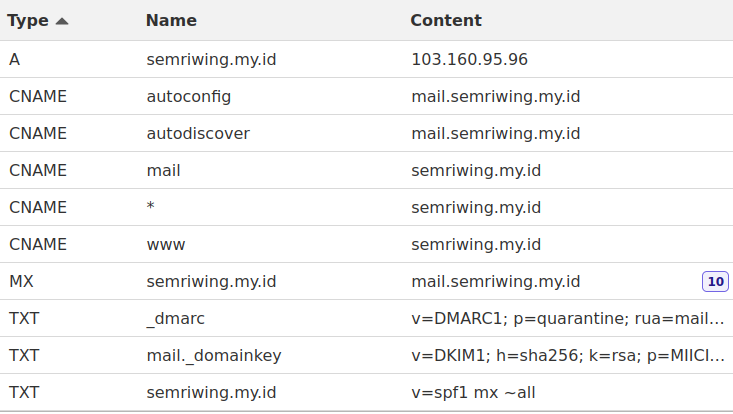
\includegraphics[width=0.95\textwidth]{dns-dkim}
        \end{center}
        \caption{Domain setelah ditambahkan subdomain DKIM}
        \label{dkim}
      \end{figure}
      \paragraph*{} Langkah selanjutnya adalah membuat DKIM
      supaya email yang dikirim dari email server yang
      dibuat tidak ditandai sebagai spam.
      Pembuatan key DKIM diharuskan
      untuk sudah membuat minimal satu akun email dari
      domain. Perintah untuk membuat key dkim adalah
      \texttt{./setup.sh config dkim}. Setelah itu 
      key dkim bisa disalin dari direktori yang di-\textit{mount}
      ke dalam container, pada penelitian ini yaitu
      \texttt{\path{dms/config/opendkim/keys/example.com/mail.txt}},
      isi dari file tersebut seperti pada gambar
      \ref{dkim_key}.
      Isi dari file tersebut disalin dan di taruh ke
      konfigurasi sub domain ``mail.\_domainkey'' seperti pada
      gambar \ref{dkim}. 

  \end{enumerate}
\end{document}
